\chapter{Market Impact and the Square-Root Law}
\label{ch:market_impact}
\chaptermark{Market impact}

Buy $1000$ shares of a liquid stock; the price moves up. Buy $2000$;
it moves up further. Kyle's linear equilibrium (\cref{ch:kyle_gm})
says twice the order, twice the impact. Real markets disagree:
thirty years of empirical evidence says impact grows as $\sqrt{Q}$,
not $Q$. Double the order, and impact grows by $\sqrt{2} \approx 1.41$.

This is not a small correction. A trader executing $5$M shares who
predicts cost from a linear model calibrated on $100{,}000$-share
trades overestimates the cost by roughly
$\sqrt{5{,}000{,}000 / 100{,}000} = \sqrt{50} \approx 7$. On a
$\$500$m parent order that is tens of basis points. Execution desks
live and die on this one law.

The \textbf{square-root law of market impact} is one of the most
robust quantitative regularities in finance. It survives across
equities, futures, FX, and options, across decades, across trade-size
scales spanning four or five orders of magnitude, and across the
break between open-outcry and electronic trading. It also contradicts
the linear impact derived in \cref{ch:kyle_gm} and assumed (for
tractability) in \cref{ch:almgren_chriss}. This chapter covers
(i)~what the law is, (ii)~three theoretical justifications,
(iii)~how it fails to match the linear textbook models, and
(iv)~how practitioners live with the contradiction.

\begin{backgroundbox}[Prerequisites]
From earlier in the book:
\begin{itemize}
  \item \Cref{ch:lob}: the limit order book, limit orders, market
  orders, the ``walking the book'' calculation for a market order
  that consumes multiple price levels, the specific toy four-level
  LOB with best bid $\bidp = 102.54$ (quantity $131$) and best ask
  $\askp = 103.23$ (quantity $48$) used throughout Part~I.
  \item \Cref{ch:spreads_roll}: the three-cause decomposition of
  the bid--ask spread into order-processing cost, inventory risk,
  and adverse selection.
  \item \Cref{ch:kyle_gm}: Kyle's (1985) linear equilibrium and the
  price-impact coefficient $\lamk = \sigma_V / (2\sigma_u)$, which
  posits that the market clearing price moves \emph{linearly} in
  the net order flow $y$. This chapter contradicts that linearity
  on empirical grounds, so the reader must know what is being
  contradicted.
\end{itemize}
From outside the book:
\begin{itemize}
  \item Basic calculus and square-root arithmetic (if the reader
  finds $\sqrt{50} \approx 7.07$ surprising, start here).
  \item Standard descriptive statistics --- mean, standard
  deviation, daily volatility. The ``$\sigma$'' in this chapter is
  always a daily return volatility unless otherwise stated.
  \item The notion of a \textbf{basis point} (bp): one hundredth of
  a percentage point, i.e.\ $1 \text{ bp} = 10^{-4}$. ``$63$ bps''
  means $0.63\%$. Every trading-cost number in this chapter is
  given in basis points so that magnitudes across asset classes
  are comparable.
\end{itemize}
\end{backgroundbox}

\section{Defining market impact}
\label{sec:defining_impact}

\emph{Market impact} has three distinct meanings; muddling them is a
common source of confusion. This section pins each one down before
stating the law that connects them.

\subsection{The basic picture}
\label{subsec:basic_picture}

A trader wants to buy a quantity $Q$. Sending it as a single market
order walks up the ask (\cref{ch:lob}); instead, the trader slices
the parent order into many small \textbf{child orders} executed over
minutes or hours, letting the market refill in between.

\begin{definition}[Metaorder]
\index{metaorder|textbf}
A \textbf{metaorder} (also called a \textbf{parent order}) is a
trading decision taken at one moment by one agent --- ``buy
$1{,}000{,}000$ shares of AAPL by the close'' --- that is then
implemented by a sequence of smaller child orders sent to the market
over an execution window of finite duration $T$. The total executed
size is~$Q$. A metaorder is atomic from the point of view of the
trader who made the decision; it is dozens or thousands of orders
from the point of view of the exchange.
\end{definition}

Three timestamps matter. Before the metaorder starts at $t_0$ the mid
is $\midp(t_0)$. At the end of execution ($t_0 + T$) it is
$\midp(t_0 + T)$. Some time later (say $t_0 + 2T$, or next morning,
after the market has absorbed the trade) the mid settles at
$\midp(t_\infty)$. The quantities of interest are the differences
between these three prices.

\begin{definition}[Temporary impact]
\index{market impact!temporary|textbf}
\label{def:temp_impact}
The \textbf{temporary impact} of a buy metaorder of size $Q$ is the
portion of the price move during execution that subsequently reverts.
Formally,
\[
  I_{\text{temp}}(Q) \;\defeq\; \midp(t_0 + T) - \midp(t_\infty).
\]
This is the short-lived liquidity premium the trader paid for
consuming visible liquidity faster than the market could replenish
it, which the market then unwinds. Temporary impact is a cost to the
initiator but not a lasting move in the underlying price.
\end{definition}

\begin{definition}[Permanent impact]
\index{market impact!permanent|textbf}
\label{def:perm_impact}
The \textbf{permanent impact} of a buy metaorder of size $Q$ is the
portion of the execution-window price move that remains after the
market has had time to absorb the trade:
\[
  I_{\text{perm}}(Q) \;\defeq\; \midp(t_\infty) - \midp(t_0).
\]
This is the information-revealing component: the market treats the
trade as a signal that fair value is higher, and updates the mid
permanently. Same mechanism as Kyle / Glosten--Milgrom
(\cref{ch:kyle_gm}): informed order flow moves the mid.
\end{definition}

\begin{definition}[Total (execution) impact]
\index{market impact!total|textbf}
\label{def:total_impact}
The \textbf{total impact}, or \emph{execution cost}, of a buy
metaorder of size $Q$ is the difference between the \emph{average
fill price} the trader achieved and the mid-price at the moment the
metaorder started:
\[
  I_{\text{tot}}(Q) \;\defeq\; \bar{p}_{\text{fill}}(Q) - \midp(t_0).
\]
This is the P\&L-relevant cost: what the trader paid relative to the
price they saw when they decided to trade. The square-root law is a
statement about $I_{\text{tot}}$.
\end{definition}

Picture the mid as a function of time during a buy metaorder: flat
before, rising during, then partly reverting after. The peak
decomposes as
\[
  \underbrace{\midp(t_0 + T) - \midp(t_0)}_{\text{peak impact}}
  \;\;=\;\;
  \underbrace{I_{\text{perm}}(Q)}_{\text{what stays}}
  \;+\;
  \underbrace{I_{\text{temp}}(Q)}_{\text{what reverts}}.
\]
On equity metaorders the permanent component is typically one-half to
two-thirds of the peak. The trader prices the metaorder using
$I_{\text{tot}}$ (it hits their P\&L); the risk manager uses
$I_{\text{perm}}$ (it sets tomorrow's mark).

\begin{figure}[ht]
\centering
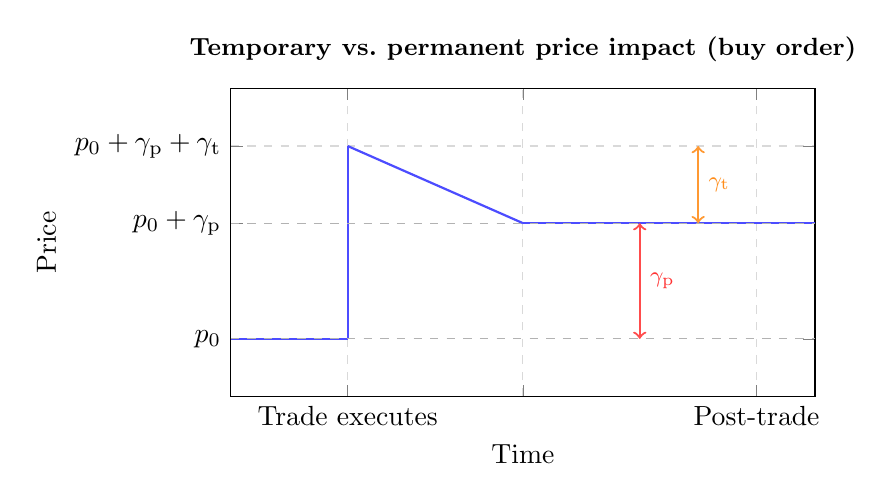
\begin{tikzpicture}
\begin{axis}[
  width=9cm, height=5.5cm,
  xlabel={Time},
  ylabel={Price},
  xmin=0, xmax=10,
  ymin=98.5, ymax=106.5,
  xtick={2,5,9},
  xticklabels={Trade executes,{},Post-trade},
  ytick={100,103,105},
  yticklabels={$p_0$, $p_0+\gamma_{\mathrm{p}}$, $p_0+\gamma_{\mathrm{p}}+\gamma_{\mathrm{t}}$},
  title={Temporary vs.\ permanent price impact (buy order)},
  title style={font=\small\bfseries},
  grid=major, grid style={dashed,gray!30},
]
\addplot[blue!70, thick] coordinates {(0,100)(2,100)};
\addplot[blue!70, thick] coordinates {(2,100)(2,105)};
\addplot[blue!70, thick] coordinates {(2,105)(5,103)};
\addplot[blue!70, thick] coordinates {(5,103)(10,103)};
\addplot[dashed, gray!60, thin] coordinates {(0,103)(10,103)};
\addplot[dashed, gray!60, thin] coordinates {(0,100)(10,100)};
\draw[<->, red!70, thick]
  (axis cs:7,100) -- (axis cs:7,103)
  node[midway, right, font=\footnotesize, red!80]{$\gamma_{\mathrm{p}}$};
\draw[<->, orange!80, thick]
  (axis cs:8,103) -- (axis cs:8,105)
  node[midway, right, font=\footnotesize, orange!90]{$\gamma_{\mathrm{t}}$};
\end{axis}
\end{tikzpicture}
\caption{Schematic of market impact for a buy order executed at $t=2$.
The price spikes by $\gamma_{\mathrm{p}} + \gamma_{\mathrm{t}}$ at execution.
The temporary component $\gamma_{\mathrm{t}}$ decays as the book replenishes.
The permanent component $\gamma_{\mathrm{p}}$ (information leakage or supply shift) persists indefinitely.}
\label{fig:impact_decomp}
\end{figure}

\subsection{Concave, linear, convex}
\label{subsec:concave_linear}

How does impact depend on trade size?

\begin{definition}[Concave impact function]
\index{market impact!concave|textbf}
\label{def:concave_impact}
An impact function $I(Q)$ is \textbf{concave} in $Q$ if, for any
$Q_1, Q_2 > 0$ and any $\lambda \in [0,1]$,
\[
  I(\lambda Q_1 + (1 - \lambda) Q_2) \;\ge\; \lambda I(Q_1) + (1-\lambda)I(Q_2).
\]
Equivalently, its graph lies above every chord. The key consequence:
for concave $I$, doubling the order size \emph{less than} doubles
the cost. Liquidity has decreasing marginal cost.
\end{definition}

Three possibilities, three pictures:

\begin{center}
\begin{tabular}{lll}
\toprule
Shape & Functional form & What it says \\
\midrule
Linear  & $I(Q) = aQ$            & Twice the order, twice the cost. \\
Concave & $I(Q) = a\sqrt{Q}$ or $aQ^{0.5\text{--}0.7}$
                                 & Twice the order, $\sqrt{2} \times$ cost. \\
Convex  & $I(Q) = aQ^2$          & Twice the order, four times the cost. \\
\bottomrule
\end{tabular}
\end{center}

Kyle (1985), reviewed in \cref{ch:kyle_gm}, derives the linear case
under Gaussian values, Gaussian noise trading, and a one-shot batch
auction. Almgren--Chriss (\cref{ch:almgren_chriss}) assumes linearity
for tractability of the calculus-of-variations problem. The convex
case has no empirical support: no asset class shows large trades
costing disproportionately more per share than small ones.

Data shows the concave case: impact scales as the square root of
trade size.

\section{The square-root law}
\label{sec:sqrt_law}

\subsection{The formula and what each symbol means}
\label{subsec:sqrt_formula}

The square-root law states that the total impact of a metaorder of
size $Q$ scales as
\begin{equation}
  I_{\text{tot}}(Q) \;\approx\; Y \cdot \sigma \cdot \sqrt{\frac{Q}{V_{\text{daily}}}}.
  \label{eq:sqrt_law}
\end{equation}
Each symbol has a precise meaning:
\begin{itemize}
  \item $I_{\text{tot}}(Q)$ is the total impact in \emph{fractional
  price units} --- i.e.\ a dimensionless return. To convert to
  absolute currency per share, multiply by the price $\midp$. To
  convert to basis points, multiply by $10{,}000$.
  \item $Y$ is a dimensionless constant depending on asset class
  and calibration window but not on $Q$. Empirical estimates fall
  in $Y \in [0.3, 1.5]$, with $Y \approx 1$ a default for mid-cap
  equities.
  \item $\sigma$ is the \textbf{daily return volatility} --- the
  standard deviation of daily close-to-close log returns, computed
  over a recent rolling window (say $60$ trading days). ``$\sigma =
  2\%$'' means a $2\%$ daily standard deviation.
  \item $Q$ is the executed size in shares (or contracts, or notional).
  \item $V_{\text{daily}}$ is the \textbf{average daily trading
  volume} in the same units as $Q$. The ratio $Q / V_{\text{daily}}$
  --- the \textbf{participation rate} or \textbf{volume fraction}
  --- is the scale-free measure of trade size relative to the market.
\end{itemize}

The law is attributed to Almgren et al.~(2005)
\citep{almgren2005direct}, who fit a large Citigroup parent-order
database and found the $Q / V_{\text{daily}}$ power consistent with
$0.5$ at high precision. The same scaling had been reported on
futures by Torre and Ferrari (BARRA, 1999). It has since been
re-verified on dozens of datasets and summarised by Bouchaud,
Bonart, Donier, and Gould \citeBouchaud.

\begin{keyfactbox}[The square-root law of market impact]
The total impact of a metaorder of size $Q$, executed over a
reasonable fraction of a trading day, scales as
\[
  \boxed{\;I_{\text{tot}}(Q) \;\approx\; Y \cdot \sigma \cdot \sqrt{\frac{Q}{V_{\text{daily}}}},\;}
\]
where $Y$ is an asset-class-specific dimensionless constant (typically
$0.3 \le Y \le 1.5$), $\sigma$ is the daily volatility, and
$V_{\text{daily}}$ is the daily traded volume. This is the central
empirical regularity of execution cost modelling. It is concave in
$Q$, holds across equities, futures, FX, and options, and
contradicts the linear-impact predictions of Kyle (1985) and the
linear-impact assumption of Almgren--Chriss (2000).
\end{keyfactbox}

Three features of \cref{eq:sqrt_law}:

\begin{enumerate}
  \item \textbf{Scale-free in $Q / V$.} Impact depends on the
  participation rate, not $Q$ absolutely. A $10$k-share trade in a
  stock with $10$M daily volume has the same impact as a $100$k-share
  trade in a stock with $100$M daily volume (all else equal) ---
  execution cost in a single liquidity-normalised coordinate across
  all stocks.
  \item \textbf{Proportional to $\sigma$.} Impact scales with the
  asset's own volatility, not its price-per-share. A penny stock and
  a blue chip at the same $\sigma$ and participation rate have the
  same impact in bps. This is the empirical analogue of ``trade where
  you can hide in the noise'' (\cref{ch:kyle_gm}).
  \item \textbf{Exponent is exactly $0.5$.} Every high-quality fit
  on equity metaorder data produces a $95\%$ confidence interval
  containing $0.5$. The exponent is $0.5$ to within the resolution
  of the data.
\end{enumerate}

\subsection{Worked numerical example}
\label{subsec:sqrt_worked}

Take a concrete stock. Suppose:
\begin{itemize}
  \item $\sigma = 2\%$ per day (a middle-of-the-road US mid-cap),
  \item $V_{\text{daily}} = 10$ million shares per day,
  \item the trader's parent order is $Q = 1$ million shares
  (a sizeable institutional trade), and
  \item $Y = 1$, our reasonable mid-cap default.
\end{itemize}
Plug in:
\begin{align*}
  \frac{Q}{V_{\text{daily}}}
  \;&=\; \frac{10^6}{10^7} \;=\; 0.10, \\[4pt]
  \sqrt{\frac{Q}{V_{\text{daily}}}}
  \;&=\; \sqrt{0.10}
  \;=\; 0.31623,  \\[4pt]
  I_{\text{tot}}
  \;&=\; 1 \cdot 0.02 \cdot 0.31623
  \;=\; 0.006325.
\end{align*}
That is a fractional impact of $0.006325$, i.e.\
\underline{$63.25$ basis points}. If the stock trades at $\$50$, the
trader pays about $\$50 \times 0.006325 \approx \$0.32$ per share
above the pre-trade mid, for a total cost of $\$316{,}000$ on the
metaorder.

A $63$-bp cost on a $1$M-share order is what a sell-side execution
desk quotes to a client before accepting the order, and what they
are measured against afterwards. Getting the scaling wrong by a
factor of $2$ is the difference between a profitable and an
unprofitable execution business.

\Cref{tab:sqrt_scaling} tabulates the predicted impact at several
trade sizes, alongside a linear-impact model calibrated to match at
$Q = 1$M shares.

\begin{table}[htbp]
\centering
\begin{tabular}{rrrr}
\toprule
$Q$ (shares) & $Q / V_{\text{daily}}$
             & Sqrt-law impact (bps)
             & Linear-impact prediction (bps) \\
\midrule
$10{,}000$   & $0.001$ & $6.32$  & $0.63$  \\
$100{,}000$  & $0.010$ & $20.00$ & $6.32$  \\
$1{,}000{,}000$ & $0.100$ & $63.25$ & $63.25$ \\
$5{,}000{,}000$ & $0.500$ & $141.42$ & $316.23$ \\
\bottomrule
\end{tabular}
\caption{Square-root versus linear-impact predictions as a function of
trade size, for a stock with $\sigma = 2\%$, $V_{\text{daily}} = 10$M
shares, $Y = 1$. The linear model is calibrated to match the
square-root prediction at $Q = 1$M shares. The two agree at the
calibration point and diverge violently away from it.}
\label{tab:sqrt_scaling}
\end{table}

Read \cref{tab:sqrt_scaling} line by line. At $10$k shares, the
linear model predicts $10\times$ less cost than reality. At $5$M
shares, it predicts $5\times$ more cost; a trader using it would
refuse a reasonable metaorder or budget for wildly pessimistic
slippage. Every row except the calibration point is wrong in the
wrong direction. Hence the practitioner compromise of
\cref{sec:kyle_contradiction}: use a calibrated linear model, but
only near the calibration point.

\begin{intuitionbox}
The square-root law says \emph{liquidity has decreasing marginal
cost}. The first shares are expensive per unit: you blow through
tight top-of-book liquidity. The last shares are cheap: participants
have had time to refill the book, bring in latent orders, and absorb
your flow into the background noise.
\end{intuitionbox}

\section{Three theoretical justifications}
\label{sec:three_justifications}

The law is empirically rock-solid but theoretically awkward. No
model derives it cleanly the way Kyle (1985) derives linear impact.
Three heuristic arguments reach $\sqrt{Q}$ from different starting
points; none is a proof, but collectively they suggest the law is a
genuine emergent feature of liquidity formation.

\subsection{Bouchaud's latent liquidity argument}
\label{subsec:bouchaud_latent}

Bouchaud et al.\ \citeBouchaud{} argue as follows. At any moment the
limit order book shows only a tiny fraction --- maybe $1\%$ --- of
the true liquidity that would match a buy order. The rest is
\textbf{latent liquidity}: orders not yet in the book because agents
are waiting, not because they do not intend to sell. Think of a
hedge fund willing to sell at the right price but unwilling to sit
with a resting limit all day.

A metaorder eats through the thin visible liquidity almost
immediately. The resulting price move is the signal that latent
sellers use to enter the book. Latent liquidity refills at a rate
proportional to the price move; steady state is reached when
consumption rate (metaorder intensity) matches backfill rate (price
move).

The algebra --- a diffusion-reaction model for the latent supply
density --- yields a steady-state impact scaling as $\sqrt{Q}$.
Supply is not fixed: new sellers enter \emph{because} the price has
moved, keeping marginal cost below linear.

Read in reverse, this explains why Kyle gets linear impact: the
one-shot auction has no time for replenishment. Bouchaud lives in
real time; replenishment is the whole story, and replenishment
concaves the impact function.

\subsection{Farmer--Gerig dimensional analysis}
\label{subsec:farmer_dimensional}

A shorter route: dimensional analysis. Impact is a fractional price
(dimensionless). The available quantities are:
\[
  Q \text{ (shares)}, \qquad
  V_{\text{daily}} \text{ (shares/day)}, \qquad
  \sigma \text{ (returns/day}^{1/2}\text{)}, \qquad
  T \text{ (execution time, days)}.
\]
The only scale-free dimensionless combinations of $Q$, $V_{\text{daily}}$,
and $T$ are $Q/(V_{\text{daily}} T)$ (the participation rate) and
$Q/V_{\text{daily}}$ (the volume fraction). The only way to build a
\emph{return} out of these dimensionless combinations and $\sigma$
(which has units of $\text{day}^{-1/2}$) is to multiply $\sigma$ by
the square root of a time. The relevant time is the execution
duration, which, for a metaorder that trades at a constant rate,
satisfies $T \propto Q/V_{\text{daily}}$. Thus
\[
  I \;\propto\; \sigma \sqrt{T}
  \;\propto\; \sigma \sqrt{Q/V_{\text{daily}}},
\]
which is the square-root law up to the dimensionless prefactor $Y$.

This argument is due to Gabaix, Gopikrishnan, Plerou and Stanley,
developed further by Farmer, Gerig and colleagues. It does not prove
the law; it says that dimensional consistency forces it on any
impact function depending only on $Q$, $V_{\text{daily}}$, and
$\sigma$. A different exponent would require an additional
dimensional scale, and no such scale appears in the data.

\subsection{Gabaix power-law informed demand}
\label{subsec:gabaix_powerlaw}

A third route, due to Gabaix et al., builds the square-root law from
the empirical fact that large institutional trade sizes follow a
power law with tail exponent $\approx 3/2$: $\mathbb{P}(\text{size} >
q) \sim q^{-3/2}$ for large $q$. These large investors are also the
Kyle-informed ones; their aggregate demand dominates realised order
flow.

Given the $3/2$ tail, what impact function makes an individual
investor's expected profit scale-invariant under rescaling of the
size distribution? Under risk-aversion and market-efficiency
assumptions detailed in the paper, the answer is $\sqrt{Q}$. The
exponent $1/2$ is tied by a self-consistency condition to the $3/2$
tail of the institutional-trade-size distribution.

Less intuitive than Bouchaud, but appealing because it predicts
\emph{two} empirical laws (trade-size distribution and impact) and
ties them together. The $3/2$ tail is itself well-established.

\begin{intuitionbox}
Common theme: \emph{the market is not a fixed stack of liquidity but
a living system that partially refills as you consume it}. Trading
triggers other participants --- latent sellers, front-runners, HFTs,
mean-reversion bots --- to absorb part of your flow. Your cost is
the fraction you had to push through before replenishment kicked in.
Under broad assumptions, that fraction scales as $\sqrt{Q}$.
\end{intuitionbox}

\section{The contradiction with Kyle and Almgren--Chriss}
\label{sec:kyle_contradiction}

How does $\sqrt{Q}$ reconcile with the two central microstructure
models --- Kyle (\cref{ch:kyle_gm}) and Almgren--Chriss
(\cref{ch:almgren_chriss}) --- that both assume linear impact?

\subsection{Kyle: linear by construction}
\label{subsec:kyle_linear_construction}

In Kyle (1985), the market clearing price satisfies
\[
  p_1 \;=\; \lamk \cdot y \;=\; \lamk \cdot (\insidx + \noiseu),
\]
with equilibrium $\lamk^\ast = \sigma_V / (2 \sigma_u)$ a strictly
positive linear coefficient on total order flow. Linearity is built
in: the ansatz restricts the market-maker's pricing rule to $p_1 =
\lamk y$, and joint normality of $V$ and $\noiseu$ makes this the
unique best response. Gaussian projection cannot produce a
$\sqrt{|y|}$ rule.

Is Kyle's linearity wrong? Kyle is a \emph{single-period} model:
one auction, one price. The square-root metaorder lives over many
periods, and repeated interaction generates concavity --- each
child order moves the price, latent liquidity enters in response,
the next child faces a partially-replenished book. Kyle is silent
on multi-period dynamics, not wrong.

Continuous-time generalisations (Kyle's own follow-up, Back, Baruch)
give a time-varying $\lamk_t$ but still linear-in-flow impact at each
instant. They do not naturally produce $\sqrt{Q}$ cumulative cost.
The distinction: $\lamk$ is an instantaneous slope; the square-root
law is an integrated cost.

\subsection{Almgren--Chriss: linear by choice}
\label{subsec:ac_linear_choice}

Almgren and Chriss \citeAC{} set up the optimal-liquidation problem:
a trader holds $X$ shares, must liquidate over $[0, T]$, and chooses
a trading rate $v(t)$ balancing expected impact cost against the
inventory-variance penalty (\cref{ch:almgren_chriss} gives the full
solution). For the variational calculation to yield a closed form,
impact must be linear in the trading rate:
\begin{align*}
  \text{permanent impact per share} \;&=\; \gamma \cdot \text{(total traded)},\\
  \text{temporary impact per share} \;&=\; \eta \cdot v(t),
\end{align*}
for constants $\gamma, \eta > 0$ ($\eta$ here is the Almgren--Chriss
temporary-impact coefficient, unrelated to the $Y$ in the square-root
law). This is a modelling choice. The paper is candid: linearity
makes the Euler--Lagrange equation separable and produces the
hyperbolic-sine optimal trajectory. Square-root impact has no clean
closed form.

So Almgren--Chriss is linear \emph{for tractability}, not because
the authors believed in linear impact --- the same compromise as
pricing a vanilla option with Black--Scholes
(\cref{ch:black_scholes}) despite fat tails and smiles.

\subsection{The practitioner's reconciliation}
\label{subsec:practitioner_reconciliation}

The industry response is the \textbf{calibration approach}. A
sell-side execution desk will:
\begin{enumerate}
  \item Use an Almgren--Chriss-style framework (closed-form optima
  are worth a lot in production).
  \item Accept that the underlying impact is square-root, not linear.
  \item Calibrate $\eta$ so the linear model matches the square-root
  law at the typical trade size. If most parent orders are $100$k
  VWAP executions, set $\eta$ so linear impact at $100$k equals the
  square-root prediction at $100$k.
  \item Trust the model only within a factor of $\sim 3$ of the
  calibration point; outside, use a direct $\sqrt{Q}$ estimate.
\end{enumerate}
The model's form is chosen for tractability, the parameter for
empirical agreement near typical trade sizes. The trader gets the
closed-form trajectory and approximately correct costs at the sizes
they execute --- but no accuracy on order-of-magnitude extrapolation.
\Cref{ch:almgren_chriss} returns to this calibration point.

\begin{pitfallbox}[Don't extrapolate linear impact outside its calibration range]
A desk calibrates its linear-impact parameter on $10$k--$100$k-share
orders, fits at the $10$k end, and ships. A client arrives with a
$5$M-share parent order. The calibrated linear model reports:
\[
  I_{\text{linear}}(5\text{M}) \;=\; \frac{5\text{M}}{10\text{k}} \cdot I_{\text{linear}}(10\text{k})
  \;=\; 500 \cdot 6.32\text{ bps} \;=\; 3160\text{ bps}.
\]
Three thousand bps. The square-root prediction is $141$ bps. The
desk quotes $22\times$ too high, loses the trade, and the client
goes to a competitor.

Symmetrically: calibrate on large trades, send a tiny one, and the
linear model predicts near-zero cost and \emph{underestimates}
aggressive-child slippage on a thin book. Extrapolating linear
impact outside its calibration range is a stealth error. Always
report the calibration range alongside the model, and switch to
$\sqrt{Q}$ outside it.
\end{pitfallbox}

\section{Temporary versus permanent impact and the reversion profile}
\label{sec:temp_perm_profile}

The square-root law tells us how total cost scales with $Q$ but not
how it decomposes into temporary and permanent parts, nor the shape
of post-trade reversion. A few robust claims hold up.

\paragraph{Permanent component is roughly two-thirds.}
Almgren et al.~(2005), on a Citigroup equity dataset, found
$60$--$70\%$ of peak impact persists indefinitely; the remaining
$30$--$40\%$ reverts within hours. A metaorder pushing the mid up
$100$ bps at execution end leaves $60$--$70$ bps permanent and the
rest decays.

\paragraph{Reversion is slow.}
Not a sharp snap-back: the temporary component decays as a power law
(not exponential), on a time scale comparable to execution duration.
A two-hour metaorder sees temporary impact decay over several hours
afterwards. Any honest cost model has to wait for reversion to
finish before measuring permanent impact.

\paragraph{Permanent impact scales the same way.}
The permanent component scales as $\sqrt{Q}$ in participation rate,
with the permanent/temporary ratio roughly constant across trade
sizes (a property of the asset, not the trade):
\[
  I_{\text{perm}}(Q) \;\approx\; \alpha \cdot Y \cdot \sigma \sqrt{Q / V_{\text{daily}}},
\]
with $\alpha \in [0.5, 0.7]$. Permanent impact is a robust multiple
of the total cost, not an independent quantity.

\paragraph{The information interpretation.}
Permanent impact measures how much information the market read into
the metaorder (\cref{ch:kyle_gm}). High permanent/temporary ratio:
the trade was read as a signal and the mid updated. Low ratio: the
trade was read as liquidity-demanding noise and the dislocation
unwound. The decomposition distinguishes ``paying for information
leakage'' (preventable by better tactics) from ``paying for
instantaneous liquidity'' (the cost of wanting to trade now).

\begin{prosperitybox}
Return to the canonical four-level toy book from \cref{ch:lob}:
\begin{center}
\begin{tabular}{cc|cc}
\toprule
\multicolumn{2}{c|}{\textbf{BID SIDE}} & \multicolumn{2}{c}{\textbf{ASK SIDE}} \\
Qty & Price & Price & Qty \\
\midrule
$131$ & $102.54$ & $103.23$ & $48$  \\
$32$  & $101.87$ & $103.98$ & $84$  \\
$293$ & $101.48$ & $104.17$ & $38$  \\
$65$  & $101.10$ & $104.75$ & $127$ \\
\bottomrule
\end{tabular}
\end{center}
Mid $\midp = 102.885$. You send a market buy for $Q = 50$ shares.
The ask side's top level has only $48$ units, so the order walks
into the second level and fills $2$ shares at $103.98$. The
average fill price is
\[
  \bar{p}_{\text{fill}}
  \;=\; \frac{48 \cdot 103.23 + 2 \cdot 103.98}{50}
  \;=\; \frac{5163.00}{50}
  \;=\; 103.26.
\]
The two concrete numbers to compare are:
\begin{itemize}
  \item \textbf{Naive top-of-book impact.} Had the trader read
  only the best ask and assumed they would get all $50$ shares
  there, they would predict an impact of $103.23 - 102.885 =
  0.345$ price units, or about $33.5$ bps.
  \item \textbf{Actual walking-the-book impact.} The true
  average fill of $103.26$ sits $0.375$ price units above the
  mid, or about $36.5$ bps.
\end{itemize}
The $3$-bp gap is the visible concavity of this book: $50$ clears
the thin top level and nicks the second.

Compare to a square-root estimate. Take $\sigma = 1\%$ and
$V_{\text{daily}} = 2000$ shares (reasonable for a Prosperity-scale
product: rounds run $10^4$--$10^5$ ticks, per-tick volumes are
$50$--$200$ shares). With $Y = 1$:
\[
  I_{\text{sqrt}} \;=\; Y \cdot \sigma \cdot \sqrt{Q / V_{\text{daily}}} \cdot \midp
  \;=\; 1 \cdot 0.01 \cdot \sqrt{50 / 2000} \cdot 102.885
  \;\approx\; 0.163,
\]
about $15.8$ bps --- less than half the walking-the-book estimate.
Normal at Prosperity scale: the square-root law is a large-sample
fit, and a single $50$-share trade against a thin four-level book
is dominated by the idiosyncratic geometry of the top two levels.
Two lessons: (i) for market orders into a thin book, do a by-hand
walking-the-book calculation; the square-root estimate is an
order-of-magnitude sanity check. (ii) When possible, post a limit
order one tick inside the spread: the first $3$ bps of this $36$-bp
estimate vanishes and is collected as fill-improvement.
\end{prosperitybox}

\section{Measuring impact: a short Python sketch}
\label{sec:measuring_sketch}

Measuring impact is harder than it looks: the realised move from
$t_0$ to $t_0+T$ mixes your impact with everything else the market
was doing. The standard fix is to benchmark against an index (or the
market-wide open-to-close drift) and then average over many trades
of similar participation rate, fitting $I = Y \sigma
\sqrt{Q/V_{\text{daily}}}$ by non-linear least squares.

On a parent-order log, that is a handful of lines. Assume a
DataFrame with columns \texttt{size}, \texttt{avg\_fill},
\texttt{pre\_mid}, \texttt{sigma\_daily}, \texttt{volume\_daily},
and \texttt{side} ($+1$ buys, $-1$ sells).

\begin{lstlisting}[caption={Fitting the square-root law to a parent-order log.}]
import numpy as np
import pandas as pd
from scipy.optimize import curve_fit

def signed_impact_bps(row):
    # Side +1 for buys, -1 for sells; impact is positive when the
    # trade pushed the price against the trader's own side.
    return 1e4 * row["side"] * (row["avg_fill"] - row["pre_mid"]) / row["pre_mid"]

df["impact_bps"] = df.apply(signed_impact_bps, axis=1)
df["part_rate"]  = df["size"] / df["volume_daily"]

# Drop the tiny and the catastrophic for robust fitting.
mask = (df["part_rate"] > 1e-4) & (df["part_rate"] < 0.5)
fit_df = df[mask]

def sqrt_law(part_rate, Y):
    return 1e4 * Y * fit_df["sigma_daily"] * np.sqrt(part_rate)

popt, pcov = curve_fit(
    sqrt_law,
    fit_df["part_rate"].values,
    fit_df["impact_bps"].values,
)
Y_hat = popt[0]
print(f"Estimated Y = {Y_hat:.3f} (asset-class constant)")
\end{lstlisting}

Comments, all mandatory in production:
\begin{itemize}
  \item The \texttt{side} multiplier ensures buys and sells are
  both measured as cost to the trader: a sell that moves price down
  is still positive impact.
  \item The participation-rate filter drops the smallest trades
  (measurement noise) and the biggest (finite-sample tail; the law
  is reliable up to $Q/V_{\text{daily}} \approx 0.3$).
  \item Fit the exponent as well: $I = Y \sigma (Q/V)^\delta$ and
  report the $95\%$ CI on $\delta$. Every large-scale study gives a
  CI containing $0.5$.
\end{itemize}

\begin{gsbox}
On a sell-side execution desk, impact models are the central input
to algorithmic execution. A junior Strat's first rotation is
typically the \textbf{transaction cost analysis} (TCA) pipeline:
ingest last week's fills, match each child to its parent-order
decision, compute realised impact against the pre-trade mid, and
compare to model prediction. Systematic biases (``we underestimate
impact on low-float stocks by $15$ bps'') feed back into monthly
recalibration.

The numbers are enormous. A rates desk hedging a newly-issued
structured note (\cref{ch:rates_derivatives}) might execute a
$\$500$m swap in an afternoon; a $2$-bp mis-estimate is $\$100{,}000$
of P\&L on one trade. Over a year, impact-model accuracy can swing
seven-figure P\&L. This is why every bank has several people working
full-time on the $Y$ constant per asset class, and why ``we match
the square-root law to within $5\%$ out of sample'' is a promotable
line.

Workflow: (i) pull last month of parent-order fills from the OMS,
(ii) compute signed impact in bps vs pre-trade mid, (iii) bucket by
product, participation rate, and volatility regime, (iv) re-fit $Y$
per bucket, (v) write a short memo on any step-change from the
previous calibration, (vi) ship the new $Y$'s to the execution
algorithm's config. Everything in this chapter is a prerequisite.
\end{gsbox}

\section{Key facts to memorise}
\label{sec:ch6_keyfacts}

\begin{itemize}
  \item \textbf{Market impact decomposes into temporary and
  permanent components.} The temporary component is the portion of
  the execution-window price move that reverts after the metaorder
  ends; the permanent component is what stays. Both scale as
  $\sqrt{Q / V_{\text{daily}}}$. Empirical estimates put permanent
  impact at roughly $60$--$70\%$ of the peak impact on equities.
  \item \textbf{The square-root law.} $I_{\text{tot}}(Q) \approx
  Y \cdot \sigma \cdot \sqrt{Q / V_{\text{daily}}}$, with $Y \in
  [0.3, 1.5]$ a dimensionless asset-class constant, $\sigma$ the
  daily return volatility, and $Q / V_{\text{daily}}$ the
  participation rate. One of the most robust empirical regularities
  in all of microstructure.
  \item \textbf{Worked example to hold in memory.} $\sigma = 2\%$,
  $V_{\text{daily}} = 10$M, $Q = 1$M, $Y = 1$. Impact $=
  0.02 \cdot \sqrt{0.1} \approx 0.006325 = 63.25$ bps. On a
  $\$50$ stock, that is about $\$316$k of cost on a $\$50$m
  parent order.
  \item \textbf{Concavity is the point.} Doubling the metaorder
  size multiplies the \emph{impact} (not cost) by $\sqrt{2} \approx
  1.41$, not $2$. Equivalently, the marginal cost of the last
  share is \emph{lower} than the marginal cost of the first share.
  \item \textbf{Three theoretical stories.} Bouchaud's latent
  liquidity (replenishment-driven), Farmer--Gerig dimensional
  analysis (scale-free from $Q$, $V$, $\sigma$), and Gabaix power-law
  informed demand (self-consistency with $q^{-3/2}$ tail). None is
  a proof, but all point to the same exponent.
  \item \textbf{Kyle gives linear impact by construction.} The
  Kyle (1985) $\lamk$ of \cref{ch:kyle_gm} is an instantaneous
  slope in a one-shot auction. Integrated over many child orders of
  a metaorder, it does \emph{not} produce $\sqrt{Q}$; the real-time
  replenishment of liquidity is what converts the linearity of a
  single-auction price rule into a concave cumulative cost.
  \item \textbf{Almgren--Chriss assumes linear impact by choice.}
  The linearity is a tractability assumption for the
  calculus-of-variations derivation in \cref{ch:almgren_chriss},
  not a claim about nature. Practitioners calibrate the linear
  coefficient so that the Almgren--Chriss model agrees with the
  square-root law at the typical trade size they execute.
  \item \textbf{Do not extrapolate linear impact outside its
  calibration window.} A linear model calibrated on small trades
  wildly \emph{overestimates} cost on large trades; one calibrated
  on large trades \emph{underestimates} cost on small aggressive
  child orders. Switch to a direct $\sqrt{Q}$ estimate outside a
  factor-of-three band around the calibration point.
  \item \textbf{Impact is scale-free in volume fraction, not shares.}
  A $10$k-share trade in a stock with $10$M daily volume has the
  same predicted impact as a $100$k-share trade in a stock with
  $100$M daily volume, at the same $\sigma$. This is why
  institutional traders think in participation rates, not absolute
  share counts.
  \item \textbf{On a sell-side desk, impact modelling is the
  core transaction-cost-analysis task.} Monthly recalibration of
  the asset-class $Y$ constant, bucketed by product and
  participation rate, is a typical Strats workflow and a standard
  junior deliverable. The tolerance on the $Y$ is measured in
  percent; the cost of being wrong is measured in $100$-thousand-dollar
  increments per large trade.
  \item \textbf{Cross-reference map.} The Kyle linear impact this
  chapter contradicts: \cref{ch:kyle_gm}. The linear-impact
  assumption this chapter flags for later repair:
  \cref{ch:almgren_chriss}. The broader story of short-horizon
  price changes driven by order flow: \cref{ch:order_flow}.
\end{itemize}

\bigskip

Together with Kyle's linear impact (\cref{ch:kyle_gm}) and the Roll
decomposition (\cref{ch:spreads_roll}), the square-root law forms a
triangle: Kyle gives the instantaneous cost of trading on
information; the square-root law gives the integrated cost of a
metaorder; Roll gives the spread decomposition into inventory,
processing, and informed flow. Holding all three at once is what
lets a quant strat read a trade log usefully. \Cref{ch:order_flow}
turns to short-horizon order-flow dynamics --- imbalance, queue
position, and order-flow signals as return predictors ---
tick-by-tick analogues of the metaorder-scale story here.
